Отвлечемся теперь от изложения материала из Сивухина, и обратимся к специализированной литературе в поисках чего-нибудь большего.
Вообще, можно дочитать этот 54 параграф, где Сивухин текстом описывает свойства и объемных голограмм тоже, можно открыт Кириченко, где это ещё снабжено и формулами. 
Здесь же я обращусь к дополнительной литературе из задавальника:\textit{Р. Кольер, Оптическая голография. – М. : Мир, 1973}.

Какие главы и параграфы взять для нашей программы:

\subsection{Условие Брегга-Вульфа}
\begin{figure}[ht]
    \centering
    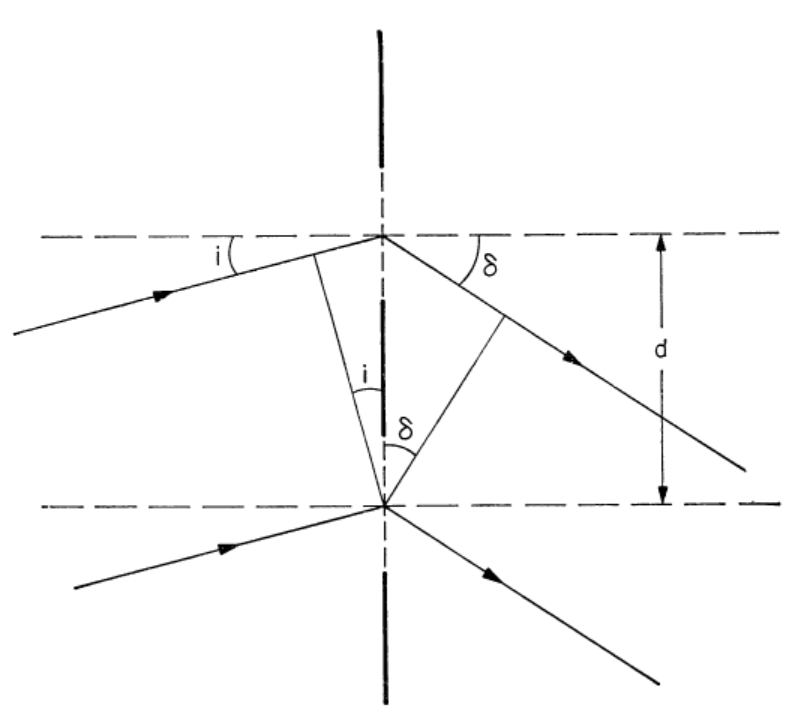
\includegraphics[width=0.4\textwidth]{figures/10_add_reshetka.png}
    \hspace{5 mm} 
    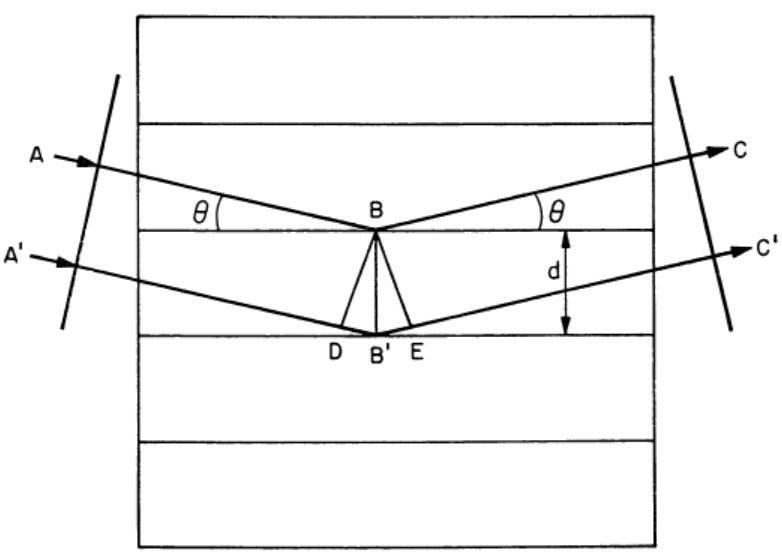
\includegraphics[width=0.4\textwidth]{figures/10_add_bregg.png}
    \caption{К формуле решетки плоской и объёменой}
    \label{fig:10_add}
\end{figure}

Помним формулу решетки, смотрим на первый рисунок, 
\begin{equation*}
	d (\sin i + \sin \delta) = \lambda,
\end{equation*}
 где ограничемся рассмотрением максимума первого порядка. 
Теперь рассмотрим второй рисунок с объемной решеткой в разрезе.
Здесь аналогично интенсивность максимальна в том направлении, в котором волны складываются симфазно.

На рисунке $DB' + B'E = 2 d \sin \theta$, что с условием максимума даёт на закон Брегга-Вульфа:
\begin{equation*}
	2 d \sin \theta = \lambda.
\end{equation*}
Таким образом получаем более жесткое условие на наблюдение максимума дифракции.
Для объёмной решетки выбор угла падения определяет и длину волны и угол дифракции. 